\documentclass[12pt,a4paper]{article}
\usepackage[utf8x]{inputenc}
\usepackage[spanish] {babel}
\usepackage{makeidx}
\usepackage[pdftex]{graphicx}

\title { \textbf{Trabajo Profesional: \\ Parallel-Editor}}
\date{2do cuatrimestre de 2010}
\author{\textbf{Ciancio Alessio, Mauro Lucas} \\
		\textbf{Gilioli, Leandro Ezequiel}	  \\
		\texttt{\{maurociancio,legilioli\}@gmail.com}
	}

\let\stdsection\section
\renewcommand\section{\newpage\stdsection}

\begin{document}
\maketitle

\begin{abstract}
En el presente trabajo se pretende encontrar y mostrar una solución al problema de
la edición concurrente de documentos en tiempo real y distribuida. Este escenario se plantea en
diversas áreas incluyendo el desarrollo de software. La técnica \textit{pair-programming} \cite{pair-programming},
generalmente propuesta por las metodologías ágiles, puede verse beneficiada al usar 
el producto que se implementa en este trabajo profesional.

Se desarrolló una solución que permite la edición simultánea de uno o más documentos, asegurando
que no exista divergencia entre las partes aún si la conexión entre ellos posee alta latencia. A su vez,
se utiliza un mecanismo optimista para modificar los documentos, en el cual no se requiere de un árbitro
central que coordine las partes involucradas.

Por último, la solución se integra con el IDE Eclipse \cite{eclipse-ide} mediante un plugin desarrollado 
para este trabajo profesional facilitando la aplicación de la técnica pair-programming.
\end{abstract}

\newpage
\tableofcontents
\newpage

\section{Presentación}

Este trabajo profesional fue desarrollado por:

	\begin{itemize}
		\item Ciancio Alessio, Mauro Lucas. \\
		      Padrón: 86.357. \\
		      \texttt{maurociancio@gmail.com}
		\item Gilioli, Leandro Ezequiel. \\
		      Padrón: 86.075. \\
   		      \texttt{legilioli@gmail.com}
	\end{itemize}

El profesor tutor de este trabajo profesional es el Lic. Pablo Cosso.

El nombre del proyecto es \texttt{Parallel-Editor} (en castellano \texttt{Editor Paralelo}) y el repositorio con la
última \textit{release} puede encontrarse en \cite{github}.

	\section{Motivación}
El desarrollo de software en sus diversas tareas ha dejado de ser un trabajo 
puramente individual y requiere interacción de varias personas que en conjunto 
suman sus capacidades para lograr un producto de calidad superior.

Bajo esta forma de trabajo es necesario disponer de herramientas que ayuden a que los tiempos
requeridos por la coordinación e interacción de los integrantes de un grupo de trabajo sean bajos
de forma tal que el grupo sea productivo.

Con este objetivo, las herramientas utilizadas deben estar diseñadas e implementadas apuntando a
integrarse con las metodologías y herramientas existentes sin representar un obstáculo para el usuario
y en lo posible, que su costo sea relativamente bajo. \\

La idea del presente trabajo profesional nace de la necesidad de participar de una sesión de desarrollo,
en la cual los participantes no están físicamente en el mismo lugar. En algunos casos en particular,
esta tarea requiere un \textit{feedback} instantáneo entre los participantes que con herramientas
existentes no se puede ofrecer.

Estas herramientas no logran que el feedback sea lo suficientemente rápido dado que trabajan
en un ambiente en el cual es necesario respetar un protocolo para la modificación del estado de un 
documento limitando la interactividad de la tarea de edición. Por ejemplo: un usuario que está trabajando
sobre un determinado archivo debe realizar todos los cambios que quiere introducir, guardar la
nueva versión del archivo modificado y enviarlo a sus colaboradores para que éstos estén al tanto de los 
cambios que introdujo (feedback). Mientras dura este proceso los colaboradores no pueden realizar cambios 
al documento y si lo hacen será necesario que realicen un proceso comúnmente llamado \textit{merge}, de forma
tal que el estado final del documento sea el mismo para cada uno de los participantes. 
En el caso en que aumenta el número de colaboradores, este proceso se hace lento y engorroso.

Este esquema funciona bien en los casos en los cuales es baja la concurrencia sobre un documento,
es decir la edición de un mismo documento por parte de más de un usuario es ocasional o en períodos de
tiempo disjuntos. Ejemplo: en el caso de que varios desarrolladores estén trabajando en un mismo proyecto 
con código fuente compartido, existen herramientas cuya efectividad está comprobada, como los sistemas de control
de versiones (entre ellos SVN, GIT, Mercurial) o servidores de archivos compartidos. \\

La solución desarrollada en este trabajo profesional se pensó para resolver los problemas que surgen
en este último caso, a saber:

\begin{itemize}
	\item Distribución geográfica: no es necesario estar en la misma ubicación física para que el proceso
	de desarrollo sea eficiente.
	\item Necesidad de un proceso de merge: el proceso de merge es realizado por el software en cada
	sitio de edición garantizando que el estado final del documento es el mismo para todos los 
	participantes. De esta manera se ahorra tiempo y se reducen los errores frecuentes o retrabajos
	los cuales son derivados de estos procesos.
	\item Alta latencia del feedback: los cambios en el estado del documento son reflejados en tiempo 
	real para todos los participantes.
\end{itemize}

La solución hace uso de tecnologías y herramientas existentes para proporcionar las funcionalidades 
que resuelven los problemas antes descriptos. Como ejemplo de esto, la solución se integró dentro de
Eclipse, el entorno de desarrollo integrado de facto para el lenguaje de programación Java.

	\section{Otras soluciones similares}
Durante la etapa de concepción del proyecto se analizaron otras soluciones similares al problema
anteriormente explicado. La descripción de cada una de ellas junto con la comparación de las mismas
respecto de la presente solución fue detallada en el documento ``Propuesta de Trabajo Profesional" 
\cite{propuestatpprof} y se muestra a continuación.

A modo de resumen se presenta el cuadro comparativo \ref{soluciones_comparacion}.

	\subsection{Google Docs \cite{googledocs} y Google Wave \cite{googlewave}}

Provee la posibilidad de editar en tiempo real concurrentemente documentos con formato utilizando
un navegador compatible. Posibilita la participación de múltiples usuarios en línea.

Sin embargo, su mayor desventaja consiste en la dependencia de una conexión a internet para la
disponibilidad del servicio. No es posible hasta ahora, la utilización del mismo en una red LAN privada.

Además es sólo utilizable a través de la interfaz web del navegador por lo cual su integración con
herramientas de terceros no es posible. Cabe aclarar que Google ha abandonado el desarrollo de Google Wave.

	\subsection{BeWeeVee \cite{beweevee}}

Framework para la integración de funcionalidades de colaboración en tiempo real en aplicaciones.
Se provee como un \textit{software development kit} para el desarrollo sobre la plataforma .NET.
Por este motivo, si bien abarca gran cantidad de desarrollos que hacen uso de dicha plataforma, no
cubre totalmente el espacio de potenciales aplicaciones ya que las aplicaciones que no se desarrollan en
.NET no pueden integrarlo.

Es de licencia libre para uso académico y aplicaciones \textit{open source}, aunque tiene un costo para
la integración en desarrollos privados.

	\subsection{COLA \cite{cola} - Eclipse Plugin}

COLA es un plugin para el IDE Eclipse que permite la colaboración en tiempo real de los usuarios para editar
un mismo documento de código fuente. Está desarrollado en Java y está basado en el proyecto Eclipse Communication
Framework (ECF). Su principal desventaja es la dependencia con el mismo y por otra parte, limita la cantidad
de usuarios que pueden participar en una sesión de edición de código a dos participantes.

	\subsection{Comparación con la presente propuesta}
El producto a desarrollar estará orientado a cubrir aquellos aspectos que las soluciones antes descriptas
dejan de lado. Se pretenden liberar el código fuente bajo una licencia open-source, garantizar la portabilidad del
mismo usando tecnologías que corren sobre la máquina virtual de Java, lograr independencia sobre otros frameworks
o componentes de software y lograr que pueda haber mas de dos participantes en la misma sesión de edición.

\begin{table}[ht]
    \begin{tabular}{ | p{2.5cm} | p{5cm} | p{5cm} | }
    \hline
    Solución & Características & Comparativa \\ \hline

    Google Docs \cite{googledocs}& Edición de documentos en tiempo real desde un navegador. &
    Sólo puede utilizarse a través de un navegador e Internet. Código fuente cerrado. \\ \hline

    Google Wave \cite{googlewave} & Comunicación y colaboración en tiempo real. &
    Ídem Google Docs. El proyecto ha sido abandonado por Google. \\ \hline

    COLA \cite{cola} (ECF) & Integración con Eclipse para colaboración en tiempo real de código fuente. &
	Limita a dos usuarios la cantidad de participantes en una sesión. Depende del proyecto ECF. \\ \hline

    BeWeeVee \cite{beweevee} & Framework para integración de funcionalidades de colaboración en tiempo real para
    la plataforma .NET. & Código fuente cerrado. Está desarrollado sólo para la plataforma .NET. \\ \hline

    \end{tabular}
    \caption{\label{soluciones_comparacion} Tabla comparativa de soluciones}
\end{table}

	\section{Justificación teórica de los algoritmos}
	
	El problema que resuelve este trabajo profesional se presenta genéricamente en escenarios en los cuales 
	existen dos o más partes que interactúan sobre un modelo (ya sea un documento o cualquier otro tipo de 
	objeto que almacene estado) aplicando operaciones sobre el mismo.
	
	Cada operación modifica el estado del modelo que es común a todas las partes. La cantidad de tipos distintos
	de operaciones que se pueden aplicar sobre el modelo depende de la naturaleza del mismo. Por ejemplo, en un
	modelo que representa un documento de texto las operaciones pueden ser inserción o borrado de texto; en el caso
	de un modelo que represente un área de dibujo se podrán aplicar operaciones de dibujado de figuras, 
	borrado, coloreado, etcétera.
	
	La existencia de varios participantes compartiendo un modelo para su edición (sucesivas aplicaciones de
	operaciones) hace que sea posible que más de un participante pueda estar realizando operaciones sobre el mismo modelo.
	Al cabo de la aplicación de cada una de ellas todos las partes deben ver el mismo estado final, es decir,
	debe ser consistente. Por esta razón hay que tener en cuenta una manera de que esta condición se garantice.

	El enfoque tradicional propone utilizar un modelo de sincronización centralizado en el cual para aplicar una
	operación sobre el modelo es necesario que el participante obtenga antes un control o autorización de un
	árbitro central. Una vez aplicada la operación, el estado resultante se transmite a todas las demás ubicaciones
	para que estén al tanto de los cambios generados como consecuencia de la aplicación de la operación remota.
	Si bien este método logra su cometido al preservar la consistencia del documento en todas las ubicaciones, la
	interactividad percibida en cada una de ellas es poco satisfactoria. Si al momento de querer aplicar una 
	operación no se tiene la autorización o control del modelo, se deberá esperar para obtenerlo. 
	Este tiempo de espera dependerá de la cantidad de participantes que se encuentran operando sobre el modelo
	en ese instante y del tiempo que cada operación remota tome en aplicarse (ejemplos de uso de este mecanismo
	son sistemas tradicionales de control de versiones con bloqueo de archivos).

	Para evitar este inconveniente y dar la impresión de una aplicación instantánea de las operaciones en cada
	una de las ubicaciones de los participantes, el \textit{modelo de la transformada operacional} (OT)
	\cite{operationaltransform} puede aplicarse. En éste, cada participante tiene una copia del modelo, sobre la
	cual aplica instantáneamente las operaciones que genera localmente. Luego de ésto, notifica el cambio a todos los demás
	participantes que forman parte del proceso colaborativo.
	Al momento en que se reciben operaciones remotas en una ubicación, estas no son aplicadas, sino que se analiza
	el tipo de operación que se recibió y la secuencia de operaciones que fueron aplicadas en esa ubicación
	anteriormente. A partir de esta información es posible transformar la operación original en otra que cumple
	la propiedad de que al aplicarse al modelo local garantiza que el estado resultante será el mismo que el de
	los modelos de todas las demás ubicaciones. \\

	El algoritmo de sincronización que se implementó fue el algoritmo de \textbf{Júpiter} \cite{jupiter}. 
	El proceso de implementación de este algoritmo se divide en varias etapas.
	
	Como primer punto es necesario definir qué tipo de componentes se va a utilizar para representar el modelo
	de documento. En esta solución se trabajará exclusivamente con el componente denominado cuadro de texto
	(\textit{textfield} en ingles). Este componente gráfico permite que se puede insertar texto en 
	posiciones definidas por el usuario y existe en la mayoría de las bibliotecas de interfaces gráficas 
	disponibles actualmente. Es posible considerar otros tipos de componentes que no se implementan en esta
	solución, como por ejemplo: una zona para dibujar entra varios usuarios, un slider, botones, checkboxes, etc.
	
	Una vez que se definieron el o los componentes es necesario definir las operaciones que podrán ser aplicadas sobre
	los mismos. Estas pueden ser definidas como las posibles modificaciones que se hacen sobre el componente.
	Por ejemplo, para el caso de cuadro de texto una posible operación es agregar el texto \textsf{``hola"} 
	en la posición 10.
	Las operaciones necesarias para modificar el estado de un documento de texto plano en el componente utilizado
	en este trabajo son	dos: agregar texto en una posición y borrar texto en una posición.
	Por razones que se explicarán más adelante, es deseable mantener la cantidad de operaciones distintas y
	la cantidad de parámetros de las mismas al mínimo.

	Por último, una vez que se definieron los componentes a utilizar y las operaciones a realizar sobre los mismos,
	la implementación del algoritmo de sincronización que fue utilizado en esta solución requiere de una función 
	de transformación de operaciones que cumple con ciertas características y se denomina
	\textit{xform } \cite{jupiter}. \\

	Para comprender la importancia de la utilización de un algoritmo de sincronización y la transformación
	de operaciones realizadas por la función \textit{xform }se procederá a plantear el siguiente escenario
	(y su descripción gráfica en la figura \ref{secuencia_ops_1}):
	
	Suponemos que dos usuarios están compartiendo un documento colaborativamente. El estado del documento 
	inicial en ambas ubicaciones es el mismo y corresponde a la palabra \texttt{"HOLA"}.
	El primer caso que se plantea como ejemplo corresponde a modificaciones al documento de manera tal 
	que las mismas no se superponen en el tiempo.
	En la ubicación 1 se inserta el carácter \texttt{'S'} en la posición 4. Esta operación se aplica localmente
	y es transmitida a la ubicación número 2. En este instante la copia local del documento es
	la palabra \texttt{"HOLAS"}.
	Mientras tanto en la ubicación 2 que posee la copia original del documento (\texttt{"HOLA"}), cuando se recibe
	la operación generada por la ubicación 1 se aplica localmente resultando ambas copias del documento idénticas.
	De igual forma en la ubicación 2 se genera otra operación (\textit{borrar carácter H}) que se aplica localmente
	y luego es transmitida a la ubicación 1. En esta se aplica la operación recibida y ambas ubicaciones terminan 
	con el mismo estado del documento.

	\begin{figure}[!ht]
		\begin{center}
			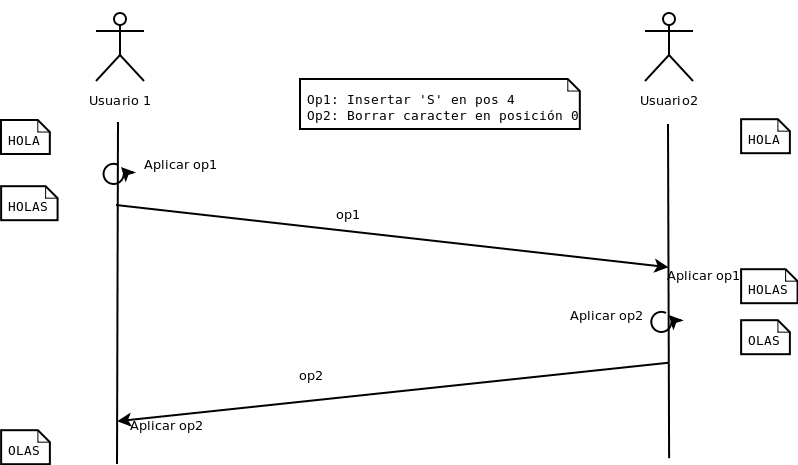
\includegraphics[width=14cm]{sincronizacion_ok.png}
			\caption{\label{secuencia_ops_1} dos ubicaciones aplican operaciones sobre el modelo }
		\end{center}
	\end{figure}

	En el caso presentado, no se observan problemas de sincronización debido a que la segunda operación fue 
	generada cuando la primera ya había sido procesada en la ubicación 2. \\

	Ahora, se presenta otro ejemplo en el que sí existe un problema de sincronización (representado en la figura
	\ref{secuencia_ops_2}). Las partes luego de procesar las operaciones tendrán documentos distintos. Esto sucede dado
	que la ubicación 2 genera una operación local sin aún haber recibido la operación generada por la otra parte.
	
	Nuevamente, el estado inicial del documento en ambas ubicaciones es \texttt{HOLA}. En la ubicación 1
	se generará la operación \textit{insertar C en posición 0} llevando el documento al estado \texttt{CHOLA}.
	Antes de que se reciba la operación en la ubicación 2, el usuario en esta ubicación generará la operación
	de borrado del carácter O. La operación es transmitida como \textit{``borrar carácter en posición 1"} ya que
	su estado actual es \texttt{HOLA}. Luego de aplicarse localmente la operación el estado del documento en
	el sitio 2 es \texttt{HLA}.
	En este momento ambas operaciones se encuentran viajando hacia las otras partes. En la ubicación 1 cuando recibe
	la operación generada remotamente, se aplica llevando al documento al estado \texttt{COLA} ya que la
	operación indicaba borrar un carácter en la posición 1. Luego, en la ubicación 2 es recibida la operación
	generada en el sitio 1. Al aplicarse localmente lleva el documento a un estado \texttt{CHLA}.
	Como se observa, en ambos sitios se observa un documento distinto.

	\begin{figure}[!ht]
		\begin{center}
			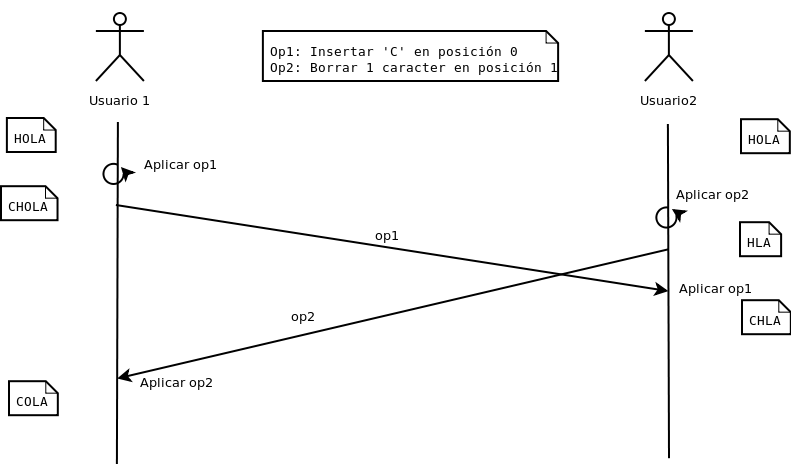
\includegraphics[width=14cm]{sincronizacion_fallida.png}
			\caption{\label{secuencia_ops_2} dos ubicaciones aplican operaciones sobre el modelo }
		\end{center}
	\end{figure}

	La divergencia en el estado final del documento se produce por que se aplicaron las operaciones en cada 
	ubicación sin haber sido transformadas previamente. En el caso de operaciones no conflictivas la función
	transformación de operaciones será la función  identidad. Sin embargo, para los casos en los cuales las
	operaciones son conflictivas la operación resultante transformada será distinta a la original.
	Para este último caso la operación 2 recibida desde la ubicación 2 debió haber sido corregida por la función
	de transformación y haber resultado en \textit{“borrar carácter en posición 2”} (y no 1 como originalmente
	era la operación).
	
	Presentada esta problemática es necesario definir una función \textit{xform} con las siguientes propiedades:
	
	\begin{equation} xform(op1,op2) = \lbrace op1’,op2’ \rbrace
	\end{equation}

	dónde \textit{op1} es la operación generada por el usuario en la ubicación 1 y \textit{op2} es la operación
	generada por el usuario en la ubicación 2. La aplicación de la función da como resultado otro par de operaciones
	\textit{op1’} y \textit{op2’} que cumplen con la propiedad de que si la ubicación 1 aplica \textit{op1} seguida
	de  \textit{op2’}  y si la ubicación 2 aplica \textit{op2} seguida de \textit{op1’}, entonces ambas
	ubicaciones terminarán con el mismo estado del documento.
	Esto requiere que \textit{op1} y \textit{op2} hayan sido generadas a partir del mismo estado del documento.

	Para el caso anterior, se mostrará a continuación la función \textit{xform}.
	Se parte del estado inicial del documento \texttt{HOLA}.

	En la ubicación 1 se aplica \textit{op1} y al momento en el que se recibe \textit{op2} se la transforma 
	para obtener la operación que debe aplicarse. A su vez, en la ubicación 2 se procede de forma similar
	aplicando primero localmente \textit{op2} y transformando \textit{op1} cuando se recibe.

	En ambas ubicaciones las operaciones transformadas se obtienen de la aplicación de \textit{xform}:
	
\begin{eqnarray*}
  xform(Insertar\ Caracter\ C\ en\ Pos\ =\ 0, \\
  Borrar\ Caracter\ en\ Pos\ =\ 1) & = & \\ 
  \lbrace Insertar\ Caracter\ C\ en\ Pos\ =\ 0, \\
  Borrar\ Caracter\ en\ Pos\ =\ 2\ \rbrace  
\end{eqnarray*}

	De aquí resulta que \textit{op1’} es \textit{Insertar Carácter C en Pos = 0} y \textit{op2’} es 
	\textit{Borrar Carácter en Pos = 2}.

\textit{op1’} resultó ser igual a \textit{op1} mientras que \textit{op2’} fue desplazada con respecto a 
\textit{op2.}

En la ubicación 1 se aplica \textit{op2’} sobre el \texttt{CHOLA} resultando en: \texttt{CHLA}.

En la ubicación 2 se aplica \textit{op1’} sobre \texttt{HLA} resultando en \texttt{CHLA}.

Nótese que aplicando las operaciones transformadas se logra la convergencia del estado del documento 
en las dos ubicaciones.

\subsection{Definición de \textit{xform}}

La definición de esta función puede resultar compleja si se toma en cuenta la cantidad de 
combinaciones de las operaciones aplicables al modelo. Por esta razón se debe mantener al mínimo la 
cantidad de operaciones para simplificar el desarrollo de la función.

La función de transformación debe contemplar los casos en las que las operaciones sean conflictivas entre 
sí. Dos operaciones \textit{op1} y \textit{op2} son conflictivas si el estado final del documento al aplicar 
primero \textit{op1} y luego \textit{op2} es distinto al que se obtiene primero \textit{op2} y luego \textit{op1}.
En el caso en que las operaciones no son conflictivas la transformación de las mismas es la transformación 
identidad.

La implementación de la función \textit{xform} en la presente solución puede observarse en la clase 
\texttt{BasicXFormStrategy}. La misma fue basada en los papers de Júpiter e INRIA \cite{inria}.

	\section{Búsqueda de la solución}

El paper Júpiter \cite{jupiter} fue la base para la implementación del algoritmo de sincronización. Este paper fue 
encontrado durante el desarrollo de la visión \cite{visiontpprof} del producto. Otros papers están basados en éste y
corrigen y proponen nuevas soluciones o correcciones.

Se detectaron problemas al utilizar operaciones de longitud mayor a uno (enfoque original que se le
dio a la implementación). En un primer momento se detectaron problemas al utilizar operaciones de borrado
de más de un carácter. Luego surgieron problemas al usar inserciones de más de un carácter. Para solucionar
este problema se convirtieron las operaciones a operaciones de un carácter.

Este cambio no posee efectos colaterales importantes. Lo que se debe tener en cuenta es convertir las
operaciones generadas por la aplicación cliente (o API gráfica) a operaciones de un carácter.

Durante el desarrollo de las pruebas se encontró un caso denominado Puzzle \cite{inria} que producía una falla en la
sincronización. Se denomina Puzzle a una combinación de estados y operaciones producidas en determinadas
ubicaciones que provoca que el algoritmo no garantice la convergencia del estado del documento para todos 
los usuarios. El paper de INRIA \cite{inria} propone una solución a este problema que demuestra formalmente las 
propiedades del algoritmo de sincronización utilizado.

Se implementaron los cambios propuestos por este paper junto con los tests para probar el correcto funcionamiento.


\subsection{Problemas enfrentados durante el desarrollo}

\begin{itemize}
	\item El lenguaje de programación \textbf{Scala} es una tecnología relativamente nueva (nacida en 2003) que
	si bien es estable cuenta con herramientas poco maduras para su desarrollo. Principalmente, los IDEs disponibles
	no son tan completos funcionalmente como lo son al desarrollar en el lenguaje Java.

	\item El desarrollo se comenzó utilizando el IDE \textbf{Eclipse} pero la funcionalidad provista era muy
	limitada por lo que se cambió al \textbf{Intellij IDEA}. Este resultó ser uno de los IDEs con mayor soporte
	para el desarrollo en Scala.

	\item \textit{Scheduling} de actores: para procesos que tienen que ver con I/O se utilizaron \textit{threads}
	para no bloquear los actores restantes. Se encontró una biblioteca llamada \textit{Akka Actors} \cite{akka} que 
	provee una mejor funcionalidad de actores, pero se decidió no cambiar a la misma ya que el proyecto estaba
	en una etapa de desarrollo avanzada, evitando demoras en el calendario. Esta biblioteca provee facilidades
	para la configuración del scheduling de los actores.

    \item Se encontró una herramienta denominada SBT \cite{sbt} (\textit{Simple Build Tool}) que agiliza la compilación
    de proyectos desarrollados en Scala, pero la transición de Maven a SBT no resultaba trivial por lo que
    se descartó. El beneficio de usar esta herramienta es que permite incrementar la velocidad de compilación
    con respecto a usar el IDE o Maven.
    
\end{itemize}

\section{Riesgos}

Los riesgos que se identificaron al inicio del proyecto se detallan a continuación:

\subsection{ID 1: Demoras en el desarrollo de las funcionalidades por la poca experiencia con Scala}
Este riesgo no se materializó, en gran parte ya que se hizo una investigación y capacitación sobre el lenguaje de
programación previamente al inicio del desarrollo. Los resultados obtenidos demuestran que fue suficiente
para afrontar el proyecto. La comunidad de programadores está en constante crecimiento y es muy activa y ayudó
durante el desarrollo con los problemas que surgieron.

\subsection{ID 2: Demoras en el desarrollo de la integración con Eclipse debido al desconocimiento de la 
arquitectura del mismo}
Se encontró que la documentación disponible de la arquitectura de Eclipse es abundante y de buena calidad por
lo cual no hubo mayores inconvenientes en la etapa de desarrollo del \textit{plugin}. Este riesgo no se se
materializó.

\subsection{ID 3: Demoras en el proyecto por la no aprobación de la propuesta de trabajo profesional}
La aprobación de la propuesta se produjo según lo planeado en el calendario, aproximadamente un mes después del
inicio del proyecto. No fue necesario cambiar el alcance del proyecto.

\subsection{ID 4: Demoras en la definición de la arquitectura produce retrabajo}
Se trabajó intensamente en una definición temprana de la arquitectura que resultó estable para el proyecto. Las
decisiones arquitecturales fueron tomadas en conjunto con todo el equipo de desarrollo y esto produjo un buen
consenso y entendimiento de la misma.

\subsection{Riesgos no relevados}
Durante el desarrollo se materializó un riesgo no contemplado originalmente. La estimación de algunas tareas dentro
de los sprints \cite{sprint} realizados estuvo muy desviada del valor real de horas hombre invertidas. Principalmente el desvío se
dio en las tareas de implementación del algoritmo de sincronización, se estimó un valor mucho menor al real (ver
\textit{Sprint Backlog 2}). El desvío fue compensado por la materialización de otro riesgo que fue la sobre estimación
de tareas dejando un margen para poder cerrar el \textit{sprint} con toda la funcionalidad convenida.
Los tres sprint realizados fueron cerrados con las tareas de mayor prioridad completas. En algunos casos se pasaron 
tareas hacia siguientes \textit{sprint}, pero estas eran de baja prioridad.

\section{Elección de las tecnologías utilizadas}

\subsection{Lenguaje de programación Scala}
En retrospectiva la elección de este lenguaje para el desarrollo de los principales módulos de la solución fue
acertada. El principal beneficio que se obtuvo fue una gran simplificación al utilizar un modelo de concurrencia
basado en actores \cite{actors1,actors2}. Este modelo abstrae al desarrollador de la complejidad de utilizar
mecanismos de sincronización y comunicación entre hilos como se realiza tradicionalmente en Java.

Por otro lado, es un lenguaje multiparadigma (Orientado a Objetos y Funcional). La ventaja de esto es que permite 
utilizar construcciones de lenguajes formales que resultan más concisas para resolver determinadas problemáticas.

El lenguaje pone el foco en la inmutabilidad de los objetos haciéndolo ideal para trabajar en ambientes concurrentes.
La sintaxis del lenguaje Scala resultó altamente expresiva y concisa. La proporción final de código fuente del trabajo
entre Scala y Java es la siguiente:

	\begin{figure}[!ht]
		\begin{center}
			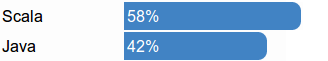
\includegraphics[width=9cm]{porcentaje.png}
			\caption{\label{porcentaje} Porcentaje de código fuente según lenguaje de programación }
		\end{center}
	\end{figure}

El lenguaje Scala es compilado a bytecode de la Java Virtual Machine. El beneficio de esto es que el código fuente
compilado de Scala es indistinguible con respecto al de Java permitiendo que los dos puedan correr en conjunto
sin problemas de compatibilidad. No existe la necesidad de codificar nuevamente bibliotecas de Java
ya que éstas pueden ser utilizadas desde Scala sin inconveniente alguno.

Teniendo en cuenta que el plugin para el IDE Eclipse fue lo único que se desarrolló en el lenguaje Java puede
notarse que comparado con éste, el código Scala es altamente denso, es decir que permite lograr gran funcionalidad 
con pocas lineas de código. El plugin fue implementado en Java debido a que el Eclipse está
implementando en este lenguaje.

Los módulos Cliente, Kernel, GUI, Common y Server fueron totalmente desarrollados en Scala.

La compatibilidad es total entre estos dos lenguajes en los dos sentidos debido a lo explicado anteriormente con
respecto al bytecode.
Este punto fue clave para el desarrollo del plugin y para la elección de Scala como lenguaje base. La misma 
resulto de gran utilidad y aceleró el proceso de desarrollo.

\subsection{IDE Eclipse}
Es el entorno integrado de desarrollo de facto para el lenguaje de programación Java y otros. La arquitectura está
basada en plugins y está concebida para que la extensión de funcionalidad sea realizada por medio de ellos. 
Posee una gran cantidad  de plugins desarrollados y una sólida documentación de la API.

Lo que se logró en el desarrollo del plugin del presente trabajo es que el mismo pueda integrarse con el IDE
y agregarle las funcionalidades sin interferir con plugins existentes. El desarrollo es compatible
con todas las funcionalidades incorporadas a los editores de texto. Por ejemplo: coloreo de código fuente, refactor,
identado, formateo, generación de código fuente.

Por otro lado, Eclipse provee un proceso de despliegue e instalación de plugins sencillo. Estos son publicados 
en Internet en cualquier servidor web y la instalación de los mismos se realiza apuntando a la URL del mismo.

\subsection{Maven}
Es una herramienta que se utiliza para controlar el ciclo de vida del proyecto en términos de compilación, testing,
resolución de dependencias y despliegue. Provee una serie de tareas que facilitan estos procedimientos que deben
repetirse continuamente en el proceso de desarrollo de un producto.

El principal beneficio de utilizar Maven es que permite hacer portable el entorno de desarrollo a nuevas estaciones
de trabajo sin un esfuerzo extra. Una vez que el proyecto está configurado correctamente (mediante la declaración en el 
archivo \texttt{pom.xml}) pueden instalarse nuevos puestos de desarrollo de forma muy sencilla. Ésto es posible
ya que las bibliotecas de las que un proyecto depende se encuentran en Internet (o en una LAN) y pueden descargarse
desde cualquier ubicación.

Su arquitectura basada en plugins permite que terceros agreguen funcionalidades son publicadas en los repositorios
de Maven.

Mediante un plugin es posible integrar Maven con proyectos desarrollados en el lenguaje Scala.

\subsection{Spring Framework}
Es un framework de código abierto para el desarrollo de aplicaciones para la plataforma Java. Spring provee soporte
para simplificar el desarrollo de diversas partes de aplicaciones enterprise. Generalmente es utilizado en
la capa de servicios para la implementación de tareas como: logging, transacciones, seguridad, etc; y también 
utilizado para el acceso a los datos.

Además, ofrece un potente mecanismo de inyección de dependencias totalmente configurable mediante archivos XML, que
permiten cambiar el comportamiento de un aplicación sin la necesidad de recompilar la misma.

Fue utilizado tanto el módulo GUI como el módulo Server. Solamente fue utilizado el mecanismo de inyección
de dependencias.

Scala es totalmente compatible con Spring ya que es compilado a bytecode de la JVM.

\subsection{GIT}
GIT es un sistema de control de versiones distribuido. No requiere de un servidor central para funcionar y permite
trabajar aún si no se posee conexión de red.

Ofrece herramientas muy poderosas para la creación de ramas de desarrollo y merge de las mismas, generación de tags, etc.

A diferencia de los sistemas de control de versiones centralizados tales como SVN o CVS, GIT almacena toda la historia
del proyecto en cada working-copy. El beneficio de ésto es que la mayoría de las operaciones que se ejecutan sobre
el repositorio no requieren del uso de la red y su aplicación es casi instantánea.

GIT fue utilizado para el desarrollo del proyecto junto con GitHub \cite{github} a modo de repositorio. GitHub es un servicio
gratuito que ofrece herramientas en la web para ver los \textit{diff} de los commits, hacer comentarios de los mismos, etc.

\subsection{JUnit \cite{junit} / EasyMock \cite{easymock} / TestNG \cite{testng} }
Estos frameworks facilitan la creación de test unitarios automatizados. Se utilizaron para verificar la correcta
implementación de las funcionalidades del producto.

Para realizar el testing de funcionalidades desarrolladas en Scala se utilizó el framework JUnit. Para Java se utilizó
el framework TestNG.

EasyMock facilita la creación de \textit{mock objects} \cite{mocks} que son útiles para aislar partes que no se desean
testear. Fue utilizado tanto en el desarrollo con Scala y con Java.

\section{Arquitectura de la solución}

\subsection{Módulos}

Como primer punto se mostrarán los componentes que conforman la solución. Está compuesto por 3 módulos principales:

\begin{itemize}
	\item \textbf{Kernel}: el módulo kernel provee los servicios de colaboración en tiempo real de documentos. En él
	se encuentran las entidades que manejan el estado de los documentos, los participantes conectados al kernel y
	qué participantes se encuentran editando qué documentos.
	
	Los documentos almacenan su estado actual de modo que pueda ser enviado a los nuevos participantes que ingresen
	a la sesión de desarrollo.
	
	Los participantes pueden comunicarse entre ellos por un canal distinto al del documento, de modo para que puedan
	organizarse	para colaborar en la edición del documento. Este servicio es denominado chat y es implementando en este módulo.
	
	Además, este módulo es capaz de determinar cuando un usuario se desconectó. Cuando este evento ocurre
	el participante es desuscripto de los documentos en los cuales estaba colaborando para que no interfiera
	con la sesión de edición.
	
	\item \textbf{Cliente}: define la API mediante la cual un cliente se conecta a un servidor colaborativo 
	y edita documentos en tiempo real. 

	La API permite crear conexiones a múltiples servidores de colaboración simultáneamente y participar
	en varias sesiones de edición en el mismo instante de tiempo.
	
	A su vez, este módulo publica las interfaces que los clientes del mismo deben implementar si se
	desea hacer uso de sus funcionalidades.
	
	Este es el módulo que utilizan las aplicaciones de terceros para incorporar las funcionalidades
	de edición colaborativa. Este módulo es utilizado tanto por el módulo GUI como por el módulo Eclipse.

	\item \textbf{Common}: este módulo es utilizado por los dos módulos anteriores para compartir tipos
	y clases. No se espera que las aplicaciones clientes incluyan este módulo directamente, sino que lo hagan
	a través del módulo Kernel y/o Cliente.
	
	En este módulo se encuentran los mensajes que utilizan los clientes y el kernel para comunicarse entre sí.
	
	Además, se encuentra la estrategia de sincronización que se utiliza para mantener el estado consistente
	de los documentos que poseen los participantes.
\end{itemize}


Además existen los siguientes módulos construidos en base a los anteriores:
\begin{itemize}
	\item \textbf{Server}: es una aplicación que crea un servicio para compartir documentos que se quieren
	editar colaborativamente a través de una red TCP/IP.
	
	Este módulo puede utilizarse si se desea un servicio de colaboración dedicado.
	
	\item \textbf{GUI}: es una aplicación cliente implementada usando Swing que ofrece la funcionalidad
	para conectarse a un servicio remoto y editar documentos existentes. Ofrece la posibilidad de compartir
	y editar documentos	en un servidor colaborativo.
	
	Fue utilizado como prototipo durante el desarrollo del proyecto para analizar las funcionalidades
	que más valor agregarían.
	
	\item \textbf{Eclipse Plugin}: integra la funcionalidades del módulo cliente y kernel dentro del IDE Eclipse.
	Hace uso tanto del módulo cliente (para conectarse a servidor de colaboración existentes) como del módulo
	o kernel (para la creación de servidores de colaboración locales).
	
	Se integra como plugin y permite la edición de archivos de texto y de código fuente	dentro del IDE aprovechando
	todas las funcionalidades ya desarrolladas por la comunidad.
\end{itemize}

Las dependencias entre los módulos puede ser observada en la figura \ref{componentes}.

	\begin{figure}[!ht]
		\begin{center}
			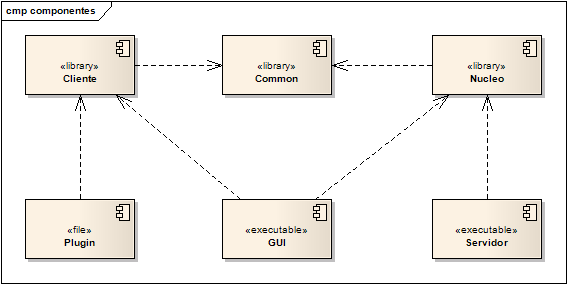
\includegraphics[width=13cm]{componentes.png}
			\caption{\label{componentes} Componentes pertenecientes a la solución y sus dependencias }
		\end{center}
	\end{figure}

\subsection{Despliegue de la solución}
Existen dos esquemas de despliegue para la solución.

\begin{itemize}
\item Cliente-Servidor
\item Peer-To-Peer
\end{itemize}

A continuación se describen las características y ventajas de cada esquema:

\subsubsection{Cliente-Servidor}
El primer caso consiste en disponer de un servidor dedicado para la gestión de documentos compartidos. El mismo recibe
peticiones de N clientes que mediante una suscripción a los documentos pueden comenzar a realizar operaciones sobre los mismos.

El servidor es el encargado de reflejar los cambios introducidos por un cliente en los restantes.

Un diagrama de esta configuración puede observarse en la figura \ref{cliente-servidor}:

	\begin{figure}[!ht]
		\begin{center}
			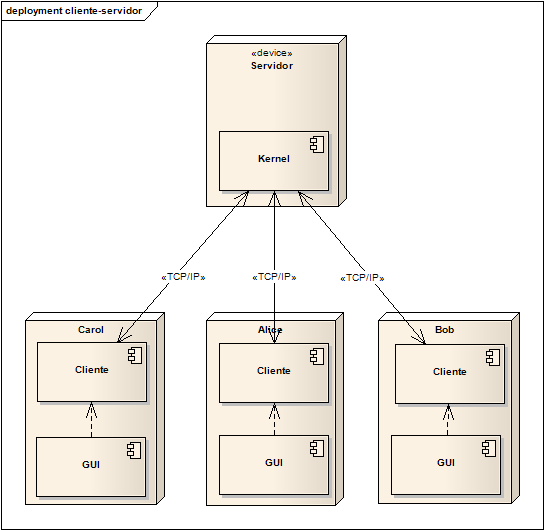
\includegraphics[width=11cm]{cliente-servidor.png}
			\caption{\label{cliente-servidor} Despliegue usando esquema cliente-servidor }
		\end{center}
	\end{figure}

Los procesos involucrados en este tipo de despliegue son:

\begin{itemize}
	\item Proceso servidor: en este proceso se encuentra ejecutándose los siguientes módulos: Kernel, Common y Server. Sólo
	hay una instancia de este proceso.
	\item Proceso cliente: en este proceso se encuentra ejecutándose los siguientes módulos: Cliente, Common y la aplicación
	correspondiente que puede ser GUI o Eclipse. La cantidad de instancias de este proceso dependen de la cantidad de usuarios que
	haya conectados al servidor de colaboración.
\end{itemize}

\subsubsection{Peer-To-Peer}
La segunda configuración para el despliegue de la solución consiste en no disponer de un servidor dedicado, sino que el
mismo es ejecutado por uno de lo pares. Este enfoque es el que se utiliza en el plugin, ya que el mismo permite crear un servicio
a partir de un archivo que se quiere compartir.

	\begin{figure}[!ht]
		\begin{center}
			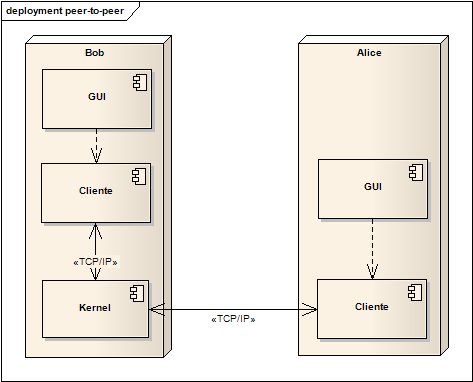
\includegraphics[width=11cm]{peer-to-peer.png}
			\caption{\label{peer-to-peer} Despliegue usando esquema peer-to-peer }
		\end{center}
	\end{figure}

Esta configuración es la más sencilla para un uso ocasional del servicio o cuando la participantes en la sesión de edición no
es elevada. Las ventajas de esta configuración es que no se necesita un equipo central.

Si los participantes se encuentran en la misma LAN, no se requiere ninguna configuración extra. Si la sesión quiere realizarse
a través de internet es necesario tener en cuenta que haya conectividad entre las partes (configuración de puertos y firewall).

Al momento de escribir esta documentación no es posible utilizar el servicio detrás de un proxy ya que los mismos
filtran todo el tráfico que no sea HTTP. En cambio si es posible hacerlo utilizarlo usando una VPN. \\

Los procesos involucrados en esta configuración son:
\begin{itemize}
	\item Proceso cliente con servicio de colaboración: Uno de los participantes involucrados será el encargado de crear el
	servicio de colaboración. En este se ejecutarán los siguientes módulos: Cliente, Kernel, Common y la aplicación que
	corresponda: GUI o Eclipse Plugin. Un sólo proceso existirá de este tipo.
	\item Procesos cliente sin servicio de colaboración: los restantes participantes se comunicarán con el cliente que posee
	el servicio de colaboración. Los módulos que se ejecutarán en este tipo de cliente son: Cliente y Common. La cantidad de
	estos procesos dependerá de la cantidad de usuarios conectados al servicio de colaboración.
\end{itemize}

Este esquema puede observarse en la figura \ref{peer-to-peer}.

\subsection{Despliegue de actores en el proceso kernel}

En la figura \ref{actores-kernel} se observan los actores desplegados en el kernel.

	\begin{figure}[!ht]
		\begin{center}
			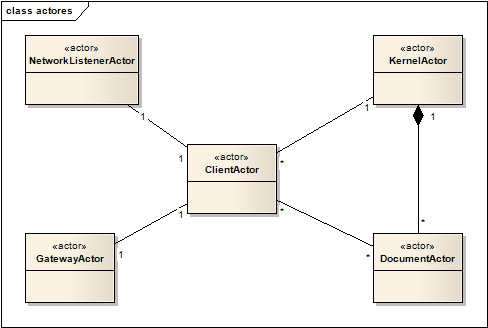
\includegraphics[width=11cm]{actores-kernel.png}
			\caption{\label{actores-kernel} Despliegue de actores en el módulo kernel }
		\end{center}
	\end{figure}

Los actores fueron utilizados para cumplir el rol de intermediario ante el acceso a un recurso, serializando los accesos de
modo de que no se produzcan conflictos de naturaleza concurrente. \\

Los principales actores del módulo kernel son los siguientes:
\begin{itemize}
	\item Kernel Actor: actúa como intermediario del objeto Kernel. La clase kernel gestiona las sesiones de los usuarios
	conectados y los documentos disponibles.
	\item Document Actor: actúa como intermediario de un objeto Document aplicando operaciones de los clientes sobre el mismo
	y replicándolas hacia los clientes restantes. Mantiene el estado del documento de modo que pueda servirlo a nuevas sesiones.
	\item Client Actor: es la representación de un cliente remoto frente al Kernel. Se encarga de recibir mensajes del
	cliente remoto, enviarlos al kernel y enviar la respuesta al mismo. Los mensajes que se reciben de la red son capturados por
	el actor NetworkListener mientras que los mensajes que se deben enviar al cliente remoto son enviados por el GatewayActor.
\end{itemize}

Existe un protocolo interno representado por los mensajes que se envían entre sí. Los mensajes que conforman este protocolo
pueden verse en el siguiente archivo: \texttt{DocumentMessages.scala}.

\subsection{Despliegue de actores en el proceso cliente}
En la figura \ref{actores-cliente} se observan los actores que se ejecutan en las aplicaciones que incorporan el módulo cliente.

	\begin{figure}[!ht]
		\begin{center}
			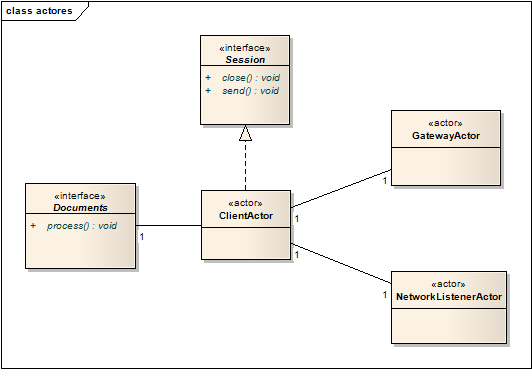
\includegraphics[width=11cm]{actores-cliente.png}
			\caption{\label{actores-cliente} Despliegue de actores en el módulo cliente }
		\end{center}
	\end{figure}

Como se observa, el esquema es similar al encontrado en el Kernel. Existe un Actor denominado ClientActor que es el
encargado de coordinar los mensajes que deben enviarse hacia el kernel y de recibir las respuestas del mismo.
Los actores NetworkListenerActor y GatewayActor son los encargados de leer y escribir mensajes por la red, respectivamente.
En el módulo cliente se define una interfaz llamada Documents que es la que debe implementar la aplicación cliente para poder
utilizar los servicios provistos por la API.
A través de esta interfaz los mensajes son propagados hacia la aplicación cliente. Es responsabilidad que la aplicación cliente
responda a estos mensajes.

Los mensajes que son enviados a la aplicación cliente pueden encontrarse en el archivo 
\texttt{ClientMessages.scala}
Con respecto a la cardinalidad de estos actores, podemos notar lo siguiente:
por cada conexión que se realiza a un servidor de colaboración es creada una instancia de cada uno de estos actores.

Cabe aclarar que estos actores se encuentran detrás de un facade, para evitar que la aplicación cliente observe la
complejidad subyacente. Este facade se denomina Session cuando es utilizado desde Scala y JSession cuando es utilizado desde Java.
Se hizo esta diferencia para que los nombres de métodos sean legibles desde Java. (Nombres de métodos que son ilegales en Java son
legales en Scala y al ser compilados a bytecode son convertidos resultando en nombres no convencionales. Ejemplo: el nombre de 
método ! es convertido a \$bang).


\subsection{Protocolo utilizado para enviar mensajes por la red}
Los mensajes son serializados e hidratados utilizando el mecanismo de serialización de objetos de Java. Los mensajes que se
envían por la red se encuentran en el archivo
\texttt{RemoteMessages.scala}.
Las clases que necesitan ser serializadas se encuentran marcadas con la anotación \texttt{@serializable}.

Se tuvo en cuenta durante la etapa de diseño que el protocolo sea fácilmente reemplazable por otro. A continuación listamos
algunas posibles razones por la cual se podría reemplazar el protocolo por otro:

\begin{itemize}
	\item Seguridad: agregar una capa que implemente cifrado de datos.
	\item Compresión: compresión de los mensajes para reducir la carga de la red.
\end{itemize}

En el archivo \texttt{SocketNetworkConnection.scala} se implementa el protocolo actual.

\subsection{Diagrama de clases del kernel}
En la figura \ref{clases-kernel} se observan las clases principales que trabajan en el Kernel. Por simplicidad no se 
incluyen métodos de determinadas clases.

	\begin{figure}[!ht]
		\begin{center}
			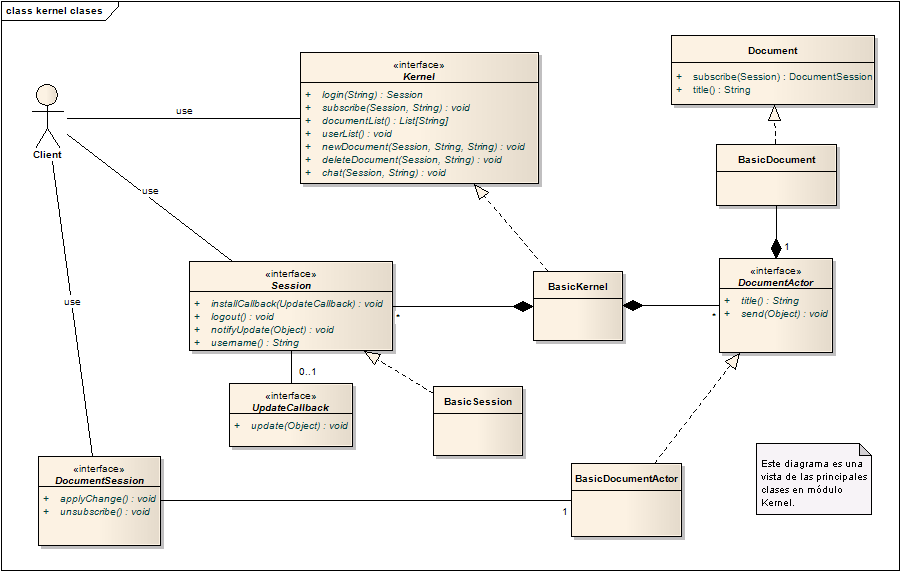
\includegraphics[width=14cm]{kernel-clases.png}
			\caption{\label{clases-kernel} Clases principales en el módulo kernel }
		\end{center}
	\end{figure}

En el mismo se muestra qué interfaces son utilizadas por los clientes. Los clientes son los usuarios que se conectan
remotamente al servicio de colaboración. Por lo tanto, el actor Cliente mostrado en el diagrama es un actor remoto y se
ocupa el rol de intermediario entre el Kernel y el Cliente real que se encuentra del otro lado de la conexión.

Las interfaces que utiliza son las siguientes:
\begin{itemize}
	\item Kernel: utiliza esta interfaz para pedir servicios al kernel de login, servicios de suscripción a documentos,
	servicios de chat, etc.

	\item Session: esta interfaz representa una sesión con el kernel. Todas las operaciones sobre el kernel requieren que se
	esté logueado al mismo. Esta interfaz ofrece la posibilidad de instalar un callback por la cual será notificada de mensajes
	provenientes del kernel. Entre estos mensajes podemos encontrar: mensajes de chat de otro usuario, mensajes de actualización
	de estado de un documento, etc. Es responsabilidad del cliente de instalar una callback para poder escuchar estos mensajes.

	\item Document Session: representa la sesión de edición de un documento en particular. Mediante esta interfaz es posible
	comunicarse con el documento para poder enviarle modificaciones.
\end{itemize}


\subsection{Circuito de mensajes y operaciones}

	\begin{figure}[!ht]
		\begin{center}
			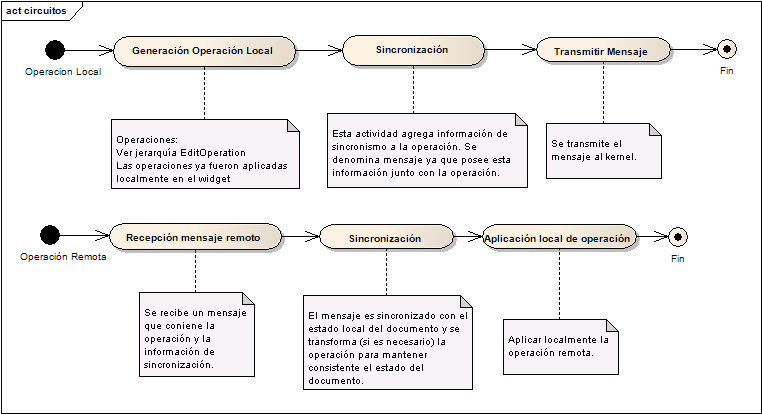
\includegraphics[width=14cm]{circuitos-mensajes.png}
			\caption{\label{circuitos-mensajes} Circuito de mensajes y operaciones }
		\end{center}
	\end{figure}


La figura \ref{circuitos-mensajes} muestra la diferencia entre mensajes y operaciones.

Notar que se reciben mensajes del kernel y sobre los widgets (o componentes) se deben aplicar operaciones. Por ese motivo es necesario 
utilizar la misma estrategia de sincronización que se utiliza en el kernel. Las clases que implementan la sincronización se 
encuentran en los archivos 
\texttt{JupiterSynchronizer.scala}
y \texttt{BasicXFormStrategy.scala}.

\subsection{Estado de Session y DocumentSession}

En la figura \ref{estado-sesion} se muestra el diagrama de estados para el login de un usuario al kernel.

	\begin{figure}[!ht]
		\begin{center}
			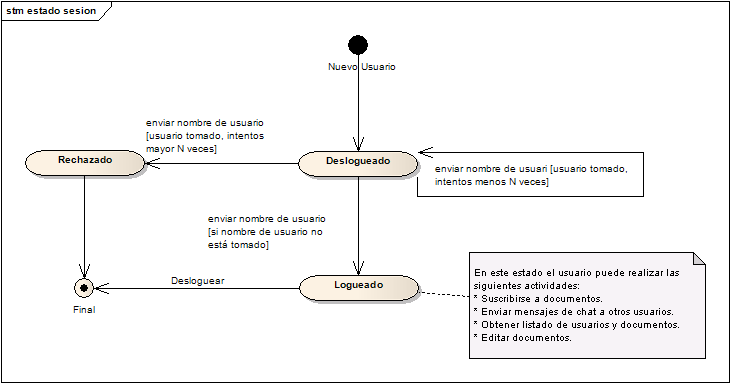
\includegraphics[width=14cm]{estado-sesion.png}
			\caption{\label{estado-sesion} Diagrama de estados de la sesión del usuario }
		\end{center}
	\end{figure}

Con el respecto a la DocumentSession, su diagrama de estados es muy sencillo. Solamente se observan dos estados, suscripto al
documento y no suscripto. Únicamente cuando se encuentra en el estado suscripto es posible aplicar operaciones sobre el mismo.
Si se trata de modificar el estado del documento cuando no se está suscripto al mismo, la operación será ignorada.

\subsection{Como integrar esta solución a productos de terceros}
Para completar la documentación sobre la arquitectura de la solución se explicará cómo integrar este producto en otros ya
existentes. Se mostrará que no es necesario rediseñar todo el producto para que pueda trabajar con Parallel-Editor.

Observaciones a tener en cuenta:

\subsubsection{API’s gráficas y Threads}

La mayoría de las API’s disponibles para hacer interfaces gráficas desktop fueron diseñadas en un 
modo no thread-safe \cite{threads-swing,threads-swt}. Es decir, que no se puede garantizar un estado 
consistente si los objetos que pertenecen a la API son accedidos desde múltiples hilos simultáneamente. 
Por esta razón, todas las actualizaciones a las ventanas, botones, widgets
en general son realizados por único thread denominado GUI Thread (o dispatching thread). Esta decisión de diseño permite que
un desarrollador no deba preocuparse en la complejidad de manejar algoritmos y estructuras de sincronización
(locks, deadlocks, etc.) que luego son difíciles de testear.

La solución desarrollada en el presente trabajo hace uso de diversos actores (que generalmente corren en un pool de threads) para poder 
responder asincrónicamente a mensajes que reciben desde el kernel. Algunos de estos mensajes requieren que se produzcan
cambios en widgets, por ejemplo al recibir un mensaje que agrega texto al sector de edición. Estos cambios deben realizarse en
el GUI Thread y no en el Thread que recibe la operación.

Generalmente, las API’s gráficas poseen mecanismos para postergar la ejecución de código para que se ejecute en el Thread de
la GUI \cite{swing-invoke-later,swt-async} y evitar los problemas de sincronización.

En la figura \ref{threads-gui} se observa el problema descripto y en la figura \ref{threads-gui-solucion} la solución.

	\begin{figure}[!ht]
		\begin{center}
			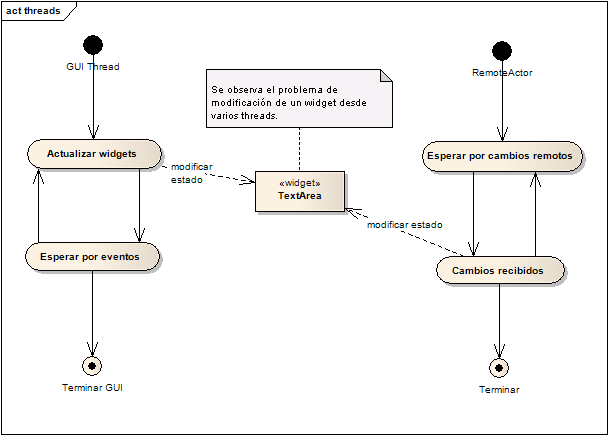
\includegraphics[width=14cm]{threads-gui.png}
			\caption{\label{threads-gui} Problemas de múltiples threads junto con el thread de la GUI }
		\end{center}
	\end{figure}


	\begin{figure}[!ht]
		\begin{center}
			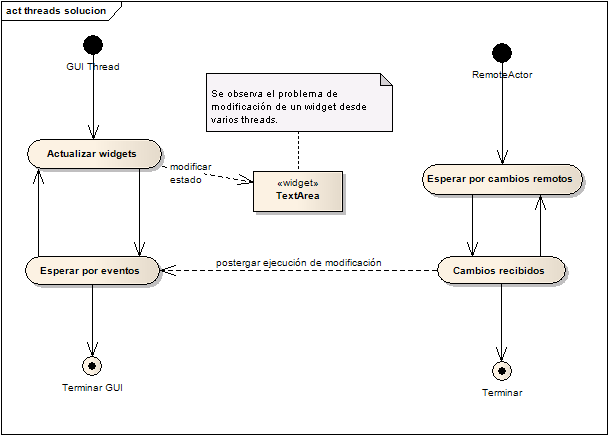
\includegraphics[width=14cm]{threads-gui-solucion.png}
			\caption{\label{threads-gui-solucion} Posible solución de múltiples threads junto con el thread de la GUI }
		\end{center}
	\end{figure}

\subsubsection{Editor de texto}
Si se desea incorporar la solución en un nuevo editor de texto (por ejemplo un IDE) es necesario tener presente 
las siguientes consideraciones:

	\begin{itemize}
		\item Se deberá implementar la interfaz \texttt{DocumentData} que ofrece un mecanismo para agregar y modificar texto en el editor. 
		A su vez ofrece un mecanismo para mantener la posición del cursor consistente y no sea movida por inserciones o
		borrado de texto por otros participantes. Si no soporta selección de texto o no existe un cursor, es posible ignorar
		las llamadas a estos métodos.
		La interfaz \texttt{DocumentData} se encuentra en el archivo \texttt{DocumentData.scala}.
		\item  Se deberá implementar un listener que atrape los eventos del widget de edición de texto y los propague al kernel.
		La mayoría de las API’s gráficas proveen un mecanismo similar.
	\end{itemize}


\subsubsection{Implementación de la interfaz Documents}
La implementación de esta interfaz se debe encargar de recibir el mensaje proveniente del kernel y si necesita realizar
cálculo intensivo, debe realizarse en otro thread. La causa de esto que el código se encontrará corriendo en el thread que
está corriendo el actor, por lo tanto, los actores deben liberar su thread para que otros actores puedan tomar su tiempo de CPU
(propiedades fairness y liveness).

\section{Metodología de desarrollo}

Scrum fue utilizado como metodología de desarrollo para llevar adelante el proyecto. La implementación de esta metodología resulto efectiva. Se alcanzaron los objetivos establecidos en la planificación en un tiempo menor 
del que se estimó en el calendario propuesto. Esto resultó así ya que durante el desarrollo del tercer sprint,
el esfuerzo dedicado al proyecto por los recursos disponibles fue mayor al que originalmente se había planificado, permitiendo completar las tareas pertenecientes al cuarto sprint durante el tercero.

El proyecto se concluyó con tres sprints en los cuales se cumplieron los objetivos detallados en el cuadro \ref{objetivos_por_sprint}.

\begin{table}
    \begin{tabular}{ | l | p{6.5cm} | p{2cm} | p{2cm} | }
    \hline
	Sprint N° & Objetivos & Fecha de Inicio & Fecha de Fin \\ \hline

	1 & Obtener un prototipo del producto con funcionalidades básicas. Definir la arquitectura del mismo con el
	objetivo de ser extendida en sprints posteriores. Los módulos afectados en este sprint son Núcleo, GUI y Cliente.
	& 13/09/2010 & 01/10/2010 \\ \hline

	2 & Extender el prototipo obtenido del sprint anterior agregándole funcionalidad de la resolución de conflictos
	generados a partir de la edición concurrente para lograr la convergencia en las partes que participan de la edición.
	Agregar funcionalidades extras a la UI para la edición de múltiples documentos simultáneamente.
	& 05/10/2010 & 29/10/2010 \\ \hline

	3 & Obtener un prototipo del plugin para el IDE Eclipse adquiriendo los conocimientos necesarios para la integración de los
	módulos en el mismo. Como objetivos secundarios se encuentran: investigación de la arquitectura de plugins para Eclipse, mejorar
	la documentación y refinar la aplicación GUI.
	& 03/11/2010 & 24/11/2010 \\ \hline

    \end{tabular}
    \caption{\label{objetivos_por_sprint} Objetivos por Sprint}
\end{table}

\subsection{Sprint 1}

Durante el primer sprint del desarrollo del presente trabajo, se puso hincapié en definir la arquitectura del mismo,
para que pueda ser extendida en sprints posteriores.

En la figura \ref{sprint1-tareas} se observan las tareas planificadas para el mismo junto que el esfuerzo empleado para
cada una de ellas.

	\begin{figure}[!ht]
		\begin{center}
			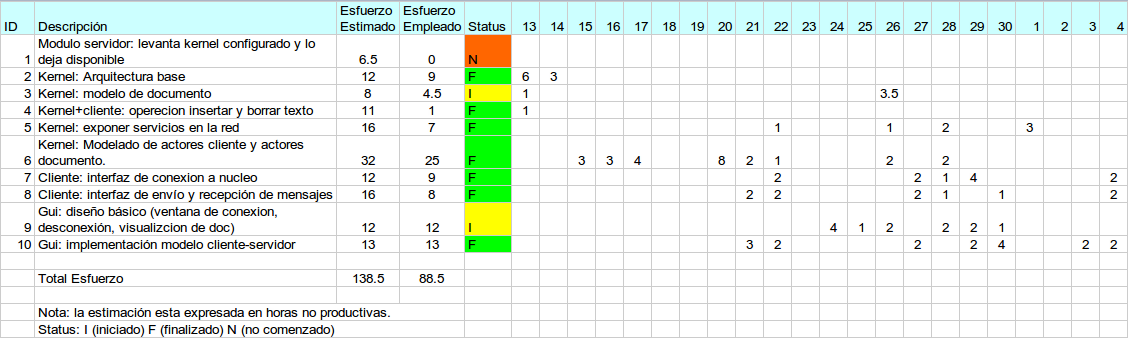
\includegraphics[width=14cm]{sprint1.png}
			\caption{\label{sprint1-tareas} Tareas planificadas para el sprint n° 1 }
		\end{center}
	\end{figure}

A continuación listaremos algunas observaciones sobre el desarrollo de este sprint:

\begin{itemize}
\item El objetivo del sprint fue alcanzado ya que se obtuvo una buena definición de la arquitectura y el prototipo
obtenido cumple con los requisitos detallados en la planificación.
\item La duración del sprint fue extendida en dos días ya que al día de cierre existían bugs críticos que no permitían
cerrar el mismo. Durante esos días extra se solucionaron esos bugs y se cerró el sprint.
\item El esfuerzo real empleado al desarrollo está muy por debajo del planificado. Se había planificado 138.5hs y se
emplearon 88.5hs. Este punto fue tenido en cuenta para los posteriores sprints.
\item Las tareas que no se cerraron en este sprint fueron planificadas para el siguiente.
\item La documentación y tests unitarios al finalizar el sprint no era la esperada, por lo que se planifican
horas para estas tareas para el siguiente sprint.
\end{itemize}

\subsection{Sprint 2}

El segundo sprint tenía por objetivo realizar una investigación sobre los algoritmo de sincronización y la implementación
de alguno de ellos en el presente trabajo. El esfuerzo empleado en este sprint fue mayor al sprint anterior y está
en el orden del planificado.

Se habían planificado 123hs y el esfuerzo empleado fue de 127.5hs.

En la figura \ref{sprint2-tareas} se observan las tareas planificadas para este sprint. Durante la planificación del
sprint se decidió agregar una columna que indique la prioridad de la tarea para poder enfocar el equipo de desarrollo
en las taras más prioritarias primero.

	\begin{figure}[!ht]
		\begin{center}
			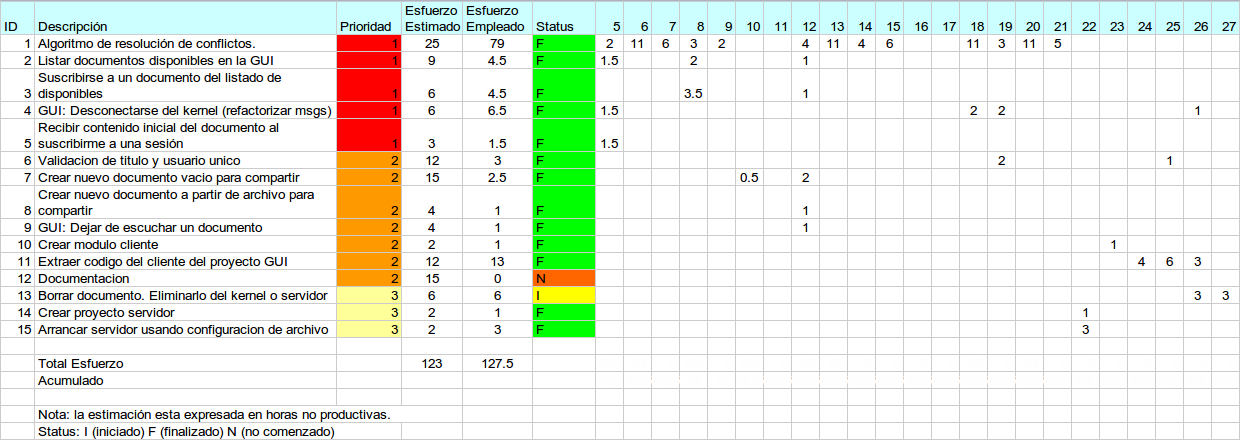
\includegraphics[width=14cm]{sprint2.png}
			\caption{\label{sprint2-tareas} Tareas planificadas para el sprint n° 2 }
		\end{center}
	\end{figure}

El las figuras \ref{sprint2-esfuerzo} y \ref{sprint2-tareas-fin} se observa el esfuerzo diario por día empleado
y el estado de las tareas al finalizar el sprint, respectivamente.

	\begin{figure}[!ht]
		\begin{center}
			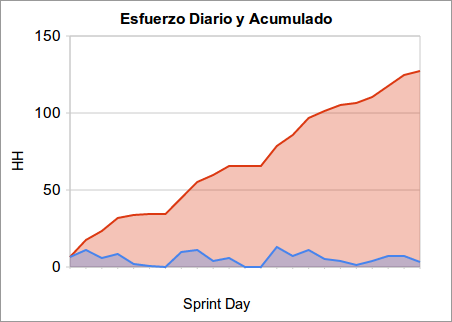
\includegraphics[width=9cm]{sprint2-esfuerzo-diario.png}
			\caption{\label{sprint2-esfuerzo} Esfuerzo diario para el sprint n° 2 }
		\end{center}
	\end{figure}

	\begin{figure}[!ht]
		\begin{center}
			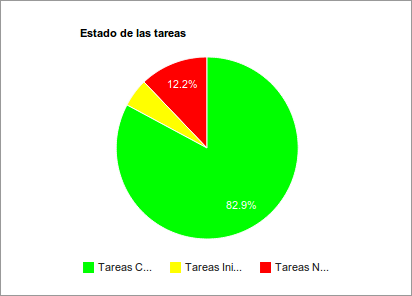
\includegraphics[width=9cm]{sprint2-tareas.png}
			\caption{\label{sprint2-tareas-fin} Estado de las tareas al finalizar el sprint n° 2 }
		\end{center}
	\end{figure}

\subsection{Sprint 3}

El objetivo del sprint tres fue integrar la solución en algún entorno de desarrollo integrado. Se decidió por el Eclipse IDE
ya que es el que más funcionalidades posee en el mundo del desarrollo de Java.

En la figura \ref{sprint3-tareas} se observa las tareas planificadas para el sprint tres. En este caso, el esfuerzo empleado
fue mayor al planificado ya que se movieron tareas pendientes para el cuarto sprint al tercero para poder cerrar la funcionalidad
sin la necesidad de un cuarto sprint.

	\begin{figure}[!ht]
		\begin{center}
			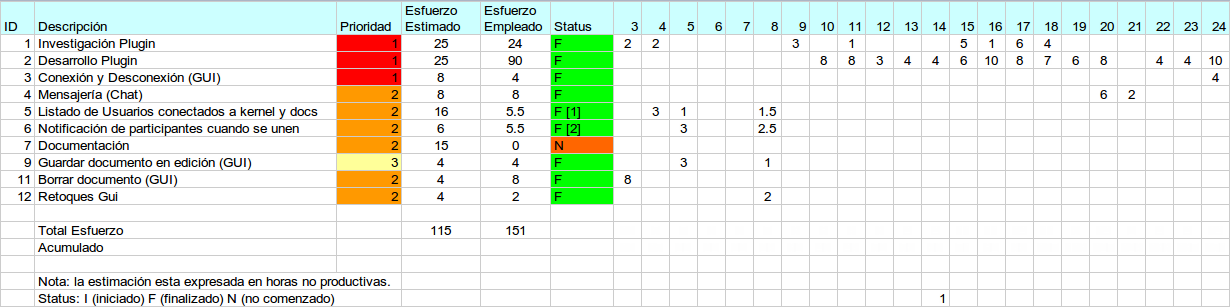
\includegraphics[width=14cm]{sprint3.png}
			\caption{\label{sprint3-tareas} Tareas planificadas para el sprint n° 3 }
		\end{center}
	\end{figure}

A su vez, se muestran en las figuras \ref{sprint3-esfuerzo} y \ref{sprint3-tareas-fin} el esfuerzo diario y el estado
de las tareas el finalizar el sprint, respectivamente.

	\begin{figure}[!ht]
		\begin{center}
			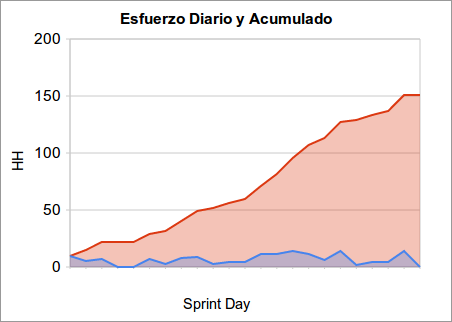
\includegraphics[width=9cm]{sprint3-esfuerzo-diario.png}
			\caption{\label{sprint3-esfuerzo} Esfuerzo diario para el sprint n° 3 }
		\end{center}
	\end{figure}

	\begin{figure}[!ht]
		\begin{center}
			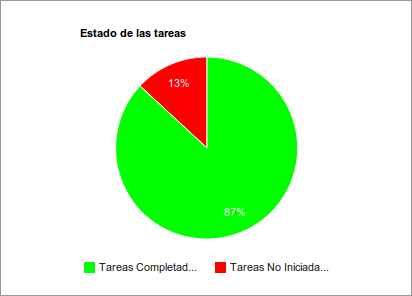
\includegraphics[width=9cm]{sprint3-tareas.png}
			\caption{\label{sprint3-tareas-fin} Estado de las tareas al finalizar el sprint n° 3 }
		\end{center}
	\end{figure}

\subsection{Otras tareas}

	Deben tenerse en cuenta en el esfuerzo total realizado unas 85 HH dedicadas a la documentación de la solución y
	confección del presente documento. Estas tareas quedaron fuera del sprint n° 3 de manera de poder cerrar la fecha del
	mismo como se había planeado originalmente.
	
	El esfuerzo total dedicado al proyecto fue de 452 HH mientras que el estimado fue de 650 HH.

	De aquí puede verse entonces que el esfuerzo total dedicado al proyecto estuvo por debajo del que 
	originalmente se había estimado y que fue detallado en el documento de Propuesta de Trabajo Profesional.

\section{Futuras líneas de investigación}

En esta sección analizaremos las futuras líneas de investigación y posibles usos de la presente solución:

\begin{itemize}
	\item Mecanismo para deshacer cambios (undo)\cite{undo1,undo2}: cuando un participante de una sesión de desarrollo se equivoca al teclear, es común
		que utilice el atajo \texttt{CTRL-Z} para deshacer su último cambio. Debe notarse que la intención del usuario es deshacer su
		último cambio y no otra posible acción realizada por otro usuario sobre el documento. Actualmente, la solución implementada
		no respeta esta intención del usuario sino que deshace el último cambio aplicado al documento independientemente de
		quién lo haya hecho. Esta mejora agrega valor al usuario y es una de las más prioritarias para próximas versiones.
		Un mecanismo de undo a implementar debería, dada una operación local ya aplicada, transformar la inversa de ésta en una nueva
		teniendo en cuenta los efectos que produjeron operaciones subsiguientes a la que se quiere deshacer de forma tal que se logre 
		el efecto deseado por el usuario al aplicarla. Esto significa que al aplicarse se eliminen los efectos de la operación que
		se quiso deshacer pero preservando las operaciones remotas que fueron aplicadas luego de la misma. La operación de undo será
		correcta si el estado alcanzado luego de aplicarla es el que se obtendría si nunca se hubiera aplicado la operación a deshacer
		pero sí las que se aplicaron luego.
		
	\item Esquema de autorización: es posible incorporar a la solución mecanismos para restringir o permitir el acceso de determinados
		usuarios a los sistema de colaboración. En muchas organizaciones existe la necesidad de auditar el trabajo de los empleados 
		por lo cual podría ser útil un registro de usuarios, que actividades realizaron, etc.

	\item Esquema de autenticación: incorporar a la solución control de acceso de usuarios permitiendo que sólo algunos
		de ellos accedan a determinados documentos.

	\item Optimización de uso de red: la reducción de la carga de red mejoraría el tiempo de respuesta de los demás participantes
		generando una sensación de mayor interactividad.

	\item Integración con otros IDEs: el plugin desarrollado en este trabajo fue implementado para el IDE Eclipse. Éste es
		actualmente uno de los más utilizado por desarrolladores en todo el mundo. La arquitectura de los módulos base fue pensada 
		para ser independiente de la aplicación que los integre. De esta forma es posible desarrollar plugins para otros entornos
		integrados de desarrollo que permiten la inclusión de los mismos como por Ej.: Intellij IDEA.

	\item Extensión de la solución para colaboración en tiempo de real sobre otros tipos de documentos:
		La solución implementada en este trabajo se limita a la colaboración en tiempo real sobre un modelo que representa
		documentos de texto. Sin embargo la teoría de la transformada operacional (OT) es aplicable a cualquier modelo de objeto en
		general. De esta manera sería posible llevar la base de la implementación de este trabajo a otros tipos de modelos. Ejemplos
		de modelos para los que se han implementado aplicaciones colaborativas son áreas de dibujo, documentos CAD y controles de
		interfaz gráfica entre otros.

	\item Cifrado de los datos: hoy en día el valor de la información es cada vez más importante dentro de las organizaciones. 
		Por este motivo debe tenerse en cuenta que si se va a utilizar una red pública o que pueda estar expuesta al monitoreo
		de terceros es sumamente importante no exponer datos sensibles en la misma sin las debidas precauciones que esto requiere.
		Bajo esta premisa sería deseable que la información transmitida por la aplicación sea enviada por la red utilizando algún
		esquema de cifrado. Esta modificación se podría implementar añadiendo una capa que encapsule el cifrado y descifrado de
		los datos, haciéndola intercambiable y transparente a la aplicación.

	\item Tráfico a través de un proxy: analizar una posible solución para que el producto pueda funcionar detrás de un
		proxy HTTP. Es muy común que en organizaciones se instalé un proxy HTTP para aumentar la performance o para
		restringir el acceso a determinados sitios. Como consecuencia se prohíbe todo el tráfico que no sea HTTP.
		
\end{itemize}

\section{Conclusiones}

Es importante simplificar el modelo que se utiliza para la programación de aplicaciones distribuidas
en tiempo real. Se requieren construcciones que separen los conceptos de infraestructura (sincronización, hilos, bloqueos, etc.)
del dominio de la aplicación. La abstracción de estos conceptos resulta clave para el desarrollo de sistemas
más comprensibles y mantenibles. Esto permite a su vez simplificar el proceso de testing o de aseguramiento
de calidad generando productos más confiables y de mayor valor para el cliente.

Aquí es dónde el modelo de concurrencia basado en Actores presenta un gran futuro. La implementación provista en la
Scala Library, que es usada en la presente solución, es completamente funcional.

Los lenguajes que hacen uso de la máquina virtual de Java (JVM) están apuntando a simplificar algunas tareas que en el lenguaje
de programación Java pueden resultar engorrosas. Entre otras características intentan aplicar el principio DRY (Don't Repeat
Yourself, en castellano No repitas) y llevan el lenguaje a un alto nivel integrando conceptos de paradigmas de 
programación que antes eran meramente de uso académico incorporándolos con éxito en el ambiente corporativo o \textit{mainstream}.
Como ejemplo se observa que la utilización de Scala en el desarrollo de este trabajo fue exitosa produciendo un código fuente
conciso y de alto nivel.

La utilización de modelos para la implementación de sistemas colaborativos de tiempo real está en plena evolución.
Existen gran cantidad de publicaciones en las cuales se presentan nuevas alternativas, agregados y mejoras a los
primeros enfoques desarrollados. Esto presenta un panorama alentador en vista de los resultados que puede tener la aplicación práctica
de estas tecnologías en el futuro cercano.

Cada vez pueden verse más aplicaciones que experimentan con la incorporación de características de colaboración en tiempo real de
forma nativa.

Estos avances y tendencias están logrando su objetivo de permitir la interacción de un grupo de trabajo de manera coordinada y
sencilla permitiendo acelerar, enriquecer y hacer más productivo su trabajo.

\section{Fuentes}

En esta sección se presenta el código fuente de las principales clases correspondientes al trabajo profesional que
son referidas a lo largo de este texto.


{
\tiny
\begin{verbatim}
package ar.noxit.paralleleditor.common.messages

import scala.serializable

/**
 * Clase base de los mensajes remotos
 */
@serializable
sealed trait BaseRemoteMessage

/**
 * Mensajes que van hacia el kernel y que deben convertirse antes de ser enviados
 */
@serializable
sealed trait ToKernel

/**
 * Mensajes enviados desde el cliente que tienen destino al kernel, son todos request
 */
@serializable
sealed trait Request

/**
 * Mensaje proveniente del kernel que son respuestas a mensajes
 */
@serializable
sealed trait Response

/**
 * Nivel documento
 */

/**
 * Clase base para las operaciones sobre documentos
 */
sealed trait RemoteOperation extends BaseRemoteMessage

/**
 * Agregar texto
 */
case class RemoteAddText(val text: String, val startPos: Int, val pword: List[Int]) extends RemoteOperation

/**
 * Borrar texto
 */
case class RemoteDeleteText(val startPos: Int, val size: Int) extends RemoteOperation

/**
 * Null operation
 */
case class RemoteNullOpText() extends RemoteOperation

/**
 * A nivel Sincronismo
 */

/**
 * información de sincronización del documento
 */
@serializable
case class SyncStatus(val myMsgs: Int, val otherMessages: Int)

/**
 * Sincronizar operaciones
 */
case class SyncOperation(val syncSatus: SyncStatus, val payload: RemoteOperation) extends BaseRemoteMessage

/**
 * A nivel kernel
 */

/**
 * Operacion sobre un determinado documento
 */
case class RemoteDocumentOperation(val docTitle: String, val payload: SyncOperation) extends BaseRemoteMessage


/**
 * Pide un nuevo documento
 */
case class RemoteNewDocumentRequest(val title: String, val initialContent: String = "") extends BaseRemoteMessage with ToKernel with Request

/**
 * Suscribirse a un doc existe
 */
case class RemoteSubscribeRequest(val title: String) extends BaseRemoteMessage with ToKernel with Request

/**
 *
 */
case class RemoteDocumentTitleExists(val offenderTitle: String) extends BaseRemoteMessage with Response

/**
 * Suscripcion aceptada
 */
case class RemoteDocumentSubscriptionResponse(val docTitle: String, val initialContent: String) extends BaseRemoteMessage with Response

/**
 * Ya existe subscripcion
 */
case class RemoteDocumentSubscriptionAlreadyExists(val offenderTitle: String) extends BaseRemoteMessage with Response

/**
 * No existe subscripcion
 */
case class RemoteDocumentSubscriptionNotExists(val offenderTitle: String) extends BaseRemoteMessage with Response

/**
 * No se puede borrar el documento, está en uso
 */
case class RemoteDocumentInUse(val docTitle: String) extends BaseRemoteMessage with Response

/**
 * El doc se borró ok
 */
case class RemoteDocumentDeletedOk(val docTitle: String) extends BaseRemoteMessage with Response

/**
 * El titulo no existe
 */
case class RemoteDocumentDeletionTitleNotExists(val docTitle: String) extends BaseRemoteMessage with Response

/**
 * Pide listado de usuarios
 */
case class RemoteUserListRequest() extends BaseRemoteMessage with Request with ToKernel

/**
 * Pide listado de documentos
 */
case class RemoteDocumentListRequest() extends BaseRemoteMessage with ToKernel with Request

/**
 * Respuesta listado de usuarios
 */
case class RemoteUserListResponse(val usernames: Map[String, List[String]]) extends BaseRemoteMessage with Response

/**
 * Respuesta de listado de documentos
 */
case class RemoteDocumentListResponse(val docList: List[String]) extends BaseRemoteMessage with Response

/**
 * Pide desuscriberse a un doc
 */
case class RemoteUnsubscribeRequest(val title: String) extends BaseRemoteMessage with Request

/**
 * Pide al kernel que borre un documento
 */
case class RemoteDeleteDocumentRequest(val docTitle: String) extends BaseRemoteMessage with Request with ToKernel

/**
 * Pide login
 */
case class RemoteLoginRequest(val username: String) extends BaseRemoteMessage with Request

/**
 * Rta de login OK
 */
case class RemoteLoginOkResponse() extends BaseRemoteMessage with Response

/**
 * Rta de Login Erroneo
 */
trait RemoteLoginRefusedRemoteResponse extends BaseRemoteMessage with Response

/**
 * Nombre de usuario tomado
 */
case class UsernameAlreadyExistsRemoteResponse() extends RemoteLoginRefusedRemoteResponse with Response

/**
 * Pedido de logout
 */
case class RemoteLogoutRequest() extends BaseRemoteMessage

/**
 * Nueva sesión iniciada
 */
case class RemoteNewUserLoggedIn(val username: String) extends BaseRemoteMessage with Response

/**
 * Sesión cerrada
 */
case class RemoteUserLoggedOut(val username: String) extends BaseRemoteMessage with Response

/**
 * Nueva suscripcion a un documento
 */
case class RemoteNewSubscriberToDocument(val username: String, val docTitle: String) extends BaseRemoteMessage with Response

/**
 * Desuscripcion a un documento
 */
case class RemoteSubscriberLeftDocument(val username: String, val docTitle: String) extends BaseRemoteMessage with Response

/**
 * desuscripcion del document ok
 */
case class RemoteSubscriptionCancelled(val docTitle: String) extends BaseRemoteMessage with Response

/**
 * Cuando no existe documento en la suscripcion
 */
case class RemoteDocumentNotExists(val offenderTitle: String) extends BaseRemoteMessage with Response

/**
 * Mensaje de chat de otro usuario
 */
case class RemoteChatMessage(val username: String, val message: String) extends BaseRemoteMessage with Response

/**
 * Send message
 */
case class RemoteSendChatMessage(val message: String) extends BaseRemoteMessage with Request with ToKernel
\end{verbatim}
}
{
\tiny
\begin{verbatim}
package ar.noxit.paralleleditor.client

import actors.Actor

/**
 * Mensajes que se envian entre un Cliente y el kernel
 */

/**
 * Le pide al kernel que lo desloguee
 */
case class Logout()

/**
 * Mensajes entre elg ClientActor y el RemoteServerProxy
 */
case class FromKernel(val msg: Any)
case class ToKernel(val msg: Any)
case class RegisterRemoteActor(val remote: Actor)

\end{verbatim}
}
{
\tiny
\begin{verbatim}
package ar.noxit.paralleleditor.kernel.messages

import ar.noxit.paralleleditor.kernel.Session
import ar.noxit.paralleleditor.common.operation.EditOperation
import ar.noxit.paralleleditor.common.Message

/**
 * Mensajes que se envian entre el actor del documento y el kernel.
 */

case class TerminateDocument()

case class ProcessOperation(val who: Session, val m: Message[EditOperation])

case class SubscriberCount()
case class Subscribe(val who: Session)
case class Unsubscribe(val who: Session)
case class SilentUnsubscribe(val session: Session)
case class Close(val session: Session)
case class DocumentDeleted(val docTitle: String)

case class DocumentUserListRequest()

case class DocumentUserListResponse(val docTitle: String, val users: List[String])

/**
 * La envia el doc actor para que el client actor la retransmita al cliente remoto
 */
case class PublishOperation(val docTitle: String, val m: Message[EditOperation])
\end{verbatim}
}
{
\tiny
\begin{verbatim}
package ar.noxit.paralleleditor.common.network

import java.net.Socket
import java.io.{ObjectOutputStream, OutputStream, ObjectInputStream, InputStream}
import ar.noxit.paralleleditor.common.logger.Loggable

class SocketNetworkConnection(private val socket: Socket) extends NetworkConnection with Loggable {
    trace("Socket network connection created")

    override def messageOutput = new SocketMessageOutput(socket.getOutputStream)

    override def messageInput = new SocketMessageInput(socket.getInputStream)

    override def close = {
        trace("Network connection closed")
        socket.close
    }
}

class SocketMessageInput(private val inputStream: InputStream) extends MessageInput {
    private val objectInput = new ObjectInputStream(inputStream)

    override def readMessage = objectInput readObject
}

class SocketMessageOutput(private val outputStream: OutputStream) extends MessageOutput {
    private val objectOutput = new ObjectOutputStream(outputStream)

    override def writeMessage(message: Any) = objectOutput writeObject message
}\end{verbatim}
}
{
\tiny
\begin{verbatim}
/*
 *  A real-time collaborative tool to develop files over the network.
 *  Copyright (C) 2010  Mauro Ciancio and Leandro Gilioli
 *                      {maurociancio,legilioli} at gmail dot com
 *
 *  This program is free software: you can redistribute it and/or modify
 *  it under the terms of the GNU General Public License as published by
 *  the Free Software Foundation, either version 3 of the License, or
 *  (at your option) any later version.
 *
 *  This program is distributed in the hope that it will be useful,
 *  but WITHOUT ANY WARRANTY; without even the implied warranty of
 *  MERCHANTABILITY or FITNESS FOR A PARTICULAR PURPOSE.  See the
 *  GNU General Public License for more details.
 *
 *  You should have received a copy of the GNU General Public License
 *  along with this program.  If not, see <http://www.gnu.org/licenses/>.
 */
package ar.noxit.paralleleditor.common

import operation._

class BasicXFormStrategy extends XFormStrategy {
    override def xform(ops: (EditOperation, EditOperation)) = {
        if (ops == null)
            throw new IllegalArgumentException("ops cannot be null")

        ops match {
            case (c: AddTextOperation, s: AddTextOperation) =>
                xform(c, s)
            case (c: DeleteTextOperation, s: DeleteTextOperation) =>
                xform(c, s)
            case (c: AddTextOperation, s: DeleteTextOperation) =>
                xform(c, s)
            case (c: DeleteTextOperation, s: AddTextOperation) =>
                xform(s, c).swap
            case (c: EditOperation, s: EditOperation) if c.isInstanceOf[NullOperation] || s.isInstanceOf[NullOperation] =>
                (c, s)
        }
    }

    /**
     * Caso agregar-agregar
     */
    protected def xform(c: AddTextOperation, s: AddTextOperation): (EditOperation, EditOperation) =
        (simpleXForm(c, s), simpleXForm(s, c))

    /**
     * Implementación según paper
     * Achieving Convergence with Operational
     * Transformation in Distributed Groupware Systems
     */
    protected def simpleXForm(c: AddTextOperation, s: AddTextOperation) = {
        if (c.text.size != 1 || s.text.size != 1) throw new UnsupportedEditOperationException("add size must be 1")

        val p1 = c.startPos
        val p2 = s.startPos
        val c1 = c.text
        val c2 = s.text
        val w1 = c.pword

        val alfa1 = pw(c)
        val alfa2 = pw(s)

        if (menor(alfa1, alfa2) || (igual(alfa1, alfa2) && c1 < c2))
            c
        else if (mayor(alfa1, alfa2) || (igual(alfa1, alfa2) && c1 > c2))
            new AddTextOperation(c1, p1 + c2.length, p1 :: w1)
        else
            c
    }

    /**
     * Caso borrar-borrar
     * para operaciones de borrado de 1 caracter
     */
    protected def xform(c: DeleteTextOperation, s: DeleteTextOperation): (EditOperation, EditOperation) = {
        if (s.size != 1 || c.size != 1) throw new UnsupportedEditOperationException("Delete size must be 1")

        val p1 = c.startPos
        val p2 = s.startPos

        if (p1 < p2)
            (c, new DeleteTextOperation(p2 - 1, s.size))
        else if (p1 > p2)
            (new DeleteTextOperation(p1 - 1, c.size), s)
        else
            (new NullOperation, new NullOperation)
    }

    /**
     * Caso agregar-borrar
     * la implementación contempla solo operaciones de borrado
     * de un caracter
     */
    protected def xform(c: AddTextOperation, s: DeleteTextOperation): (EditOperation, EditOperation) = {
        if (c.text.size != 1) throw new UnsupportedEditOperationException("add size must be 1")
        if (s.size != 1) throw new UnsupportedEditOperationException("Delete size must be 1")

        val p1 = c.startPos
        val p2 = s.startPos
        val pw = c.pword

        if (p1 > p2)
            (new AddTextOperation(c.text, p1 - 1, p1 :: pw), s)
        else if (p1 < p2)
            (c, new DeleteTextOperation(p2 + c.text.length, s.size))
        else
            (new AddTextOperation(c.text, p1, p1 :: pw), new DeleteTextOperation(p2 + c.text.length, s.size))
    }

    /**
     * público para testing
     */
    def pw(op: EditOperation) = {
        op match {
            case at: AddTextOperation => {
                // primer caso si w == vacio, con w = pword
                val p = at.startPos
                val w = at.pword

                if (w.isEmpty)
                    List(p)
                else if (!w.isEmpty && (p == current(w) || (p - current(w)).abs == 1))
                    p :: w
                else
                    List()
            }
            case dt: DeleteTextOperation => {
                val p = dt.startPos
                List(p)
            }
            case o: NullOperation => List()
        }
    }

    protected def current(pword: List[Int]) = pword.head

    private def getRangeFor(o: DeleteTextOperation) = o.startPos to (o.startPos + o.size)

    def menor(a: List[Int], b: List[Int]) = comparar(a, b, {(v1, v2) => v1 < v2})

    def mayor(a: List[Int], b: List[Int]) = comparar(a, b, {(v1, v2) => v1 > v2})

    def igual(a: List[Int], b: List[Int]) = comparar(a, b, {(v1, v2) => v1 == v2})

    private def comparar(a: List[Int], b: List[Int], comp: (Int, Int) => Boolean) = {
        val tuples = a zip b
        val result = tuples.dropWhile {t => t._1 == t._2}
        if (result isEmpty)
        // aca una es mas larga q la otra
            comp(a.size, b.size)
        else {
            val head = result.head
            comp(head._1, head._2)
        }
    }
}
\end{verbatim}
}
{
\tiny
\begin{verbatim}
/*
 *  A real-time collaborative tool to develop files over the network.
 *  Copyright (C) 2010  Mauro Ciancio and Leandro Gilioli
 *                      {maurociancio,legilioli} at gmail dot com
 *
 *  This program is free software: you can redistribute it and/or modify
 *  it under the terms of the GNU General Public License as published by
 *  the Free Software Foundation, either version 3 of the License, or
 *  (at your option) any later version.
 *
 *  This program is distributed in the hope that it will be useful,
 *  but WITHOUT ANY WARRANTY; without even the implied warranty of
 *  MERCHANTABILITY or FITNESS FOR A PARTICULAR PURPOSE.  See the
 *  GNU General Public License for more details.
 *
 *  You should have received a copy of the GNU General Public License
 *  along with this program.  If not, see <http://www.gnu.org/licenses/>.
 */
package ar.noxit.paralleleditor.common

import logger.Loggable
import operation.EditOperation

case class Message[Op](val op: Op, val myMsgs: Int, val otherMsgs: Int)

abstract class JupiterSynchronizer[Op] extends Loggable {
    /**
     * nº de  mensajes originados localmente
     */
    private var _myMsgs = 0

    /**
     * nº de  mensajes que llegaron del afuera
     */
    private var _otherMsgs = 0

    /**
     * lista de mensajes que se generaron y enviaron localmente
     */
    private var outgoingMsgs = Map[Int, Op]()

    /**
     * Getter para testing
     */
    def myMsgs = _myMsgs

    /**
     * Getter para testing
     */
    def otherMsgs = _otherMsgs

    /**
     * La operación ya fue aplicada antes de llamarse a este método
     */
    def generate(op: Op, send: Message[Op] => Unit) {
        trace("Generating message")

        // enviar mensaje a la otra parte
        send(Message(op, _myMsgs, _otherMsgs))

        outgoingMsgs = outgoingMsgs.updated(_myMsgs, op)
        _myMsgs = _myMsgs + 1

        trace("estado actual %d %d", _myMsgs, _otherMsgs)
    }

    def receive(message: Message[Op], apply: Op => Unit) {
        trace("Message received " + message)

        // filtro mensajes anteriores al recibido (acknowledged messages)
        outgoingMsgs = outgoingMsgs filterKeys (_ >= message.otherMsgs)

        val ordenedMsgs = outgoingMsgs.toArray.sortBy {_._1}

        trace("original op %s", message.op)
        // calculo la transformada de la operacion a realizar
        val finalOp = (message.op /: ordenedMsgs) {
            (transformedOp, currentListElement) => {
                val currentOp = currentListElement _2
                val transformatedOps = xform(currentOp, transformedOp)

                outgoingMsgs = outgoingMsgs.updated(currentListElement _1, transformatedOps _1)

                transformatedOps _2
            }
        }
        trace("fixed op %s", finalOp)
        apply(finalOp)

        _otherMsgs = _otherMsgs + 1
        trace("estado actual %d %d", _myMsgs, _otherMsgs)
    }

    protected def xform(c: Op, s: Op): (Op, Op)
}

class EditOperationJupiterSynchronizer(private val xformStrategy: XFormStrategy) extends JupiterSynchronizer[EditOperation] {
    override protected def xform(c: EditOperation, s: EditOperation) = xformStrategy.xform(c, s)
}

trait SendFunction {
    def send(message: Message[EditOperation])
}

trait ApplyFunction {
    def apply(operation: EditOperation)
}

class JEditOperationJupiterSynchronizer(val adaptedSync: JupiterSynchronizer[EditOperation]) {
    def generate(op: EditOperation, fun: SendFunction) =
        adaptedSync.generate(op, {m => fun.send(m)})

    def receive(message: Message[EditOperation], fun: ApplyFunction) =
        adaptedSync.receive(message, {op => fun.apply(op)})
}
\end{verbatim}
}
{
\tiny
\begin{verbatim}
package ar.noxit.paralleleditor.common.operation

trait Caret {
    def offset: Int
    def selectionLength: Int
    def change(offset: Int, selectionLength: Int)
}

trait DocumentData {
    def data: String
    def replace(offset: Int, length: Int, newText: String)
    val caret: Caret
}
\end{verbatim}
}


\newpage
\begin{thebibliography}{9}
	\bibitem{pair-programming}
	Pair-Programming. \\
	\textsl{http://en.wikipedia.org/wiki/Pair\_programming}.

	\bibitem{eclipse-ide}
	Eclipse IDE. \\
	\textsl{http://www.eclipse.org/}.

	\bibitem{visiontpprof}
	Ciancio, Gilioli,
	\emph{Visión Trabajo Profesional}.
	Facultad de Ingeniería.
	Universidad de Buenos Aires. 

	\bibitem{propuestatpprof}
	Ciancio, Gilioli,
	\emph{Propuesta de Trabajo Profesional - Paralell Editor}.
	Facultad de Ingeniería.
	Universidad de Buenos Aires. 

	\bibitem{inria}
	Imine, Molli, Oster, Rusinowitch
	\emph{Achieving Convergence With Operational Transformation in Distributed Groupware Systems}.
	Institut National de Recherche en Informatique et en Automatique.
	Rapport de recherche n° 5188. 
	Mayo 2004.

	\bibitem{jupiter}
	Nichols, Curtis, Dixon and Lamping,
	\emph{High-Latency, Low-Bandwidth Windowing in the Jupiter Collaboration System}.
	Xerox Palo Alto Research Center.

	\bibitem{actors1}
	Haller and Odersky.
	\emph{Actors That Unify Threads and Events.}
	Programming Methods Lab (LAMP).
	École Polytechnique Fédérale de Lausanne (EPFL).
	Switzerland.
 
 	\bibitem{actors2}
	Haller and Odersky.
	\emph{Event-Based Programming without Inversion of Control.}
	Programming Methods Lab (LAMP).
	École Polytechnique Fédérale de Lausanne (EPFL).
	Switzerland.

	\bibitem{operationaltransform}
	Wang, Mash and Lassen
	\emph{Google Wave Operational Transformation}.
	Versión: 1.1.
	Julio 2010.

	\bibitem{undo1}
	C. Sun.
	\emph{Undo as concurrent inverse in group editors}
	ACM Transactions on Computer-Human Interaction
	Vol. 9, No. 4, pp. 309 – 361,
	Diciembre. 2002.

	\bibitem{undo2}
	D. Sun, C. Sun
	\emph{Context-based Operational Transformation in Distributed Collaborative Editing Systems}
	IEEE Transactions on Parallel and Distributed Systems
	Vol. 20, No. 10, pp. 1454 – 1470,
	Octubre. 2009.
		
	\bibitem{googledocs}
	\emph{Google Docs}. 
	Google Inc., 
	\textsl{http://docs.google.com}.
	
	\bibitem{googlewave}
	\emph{Google Wave}. Google Inc., 
	\textsl{http://wave.google.com}.

	\bibitem{beweevee}
	Corvalius,
	\emph{BeWeeVee}. 
	\textsl{http://www.beweevee.com}.
	
	\bibitem{cola}
	Mustafa K. Isik,
	\emph{COLA}. 
	\textsl{ http://wiki.eclipse.org/RT\_Shared\_Editing}.

	\bibitem{scala}
	Venkat Subramaniam,
	\emph{Programming Scala: Tackle Multi-Core Complexity on the Java Virtual Machine}.
	Pragmatic Bookshelf, ISBN: 193435631X.
	Julio 2009.

	\bibitem{scrum}
	Ken Schwaber,
	\emph{Agile Software Development with Scrum}.
	Prentice Hall, 
	Octubre 2001.

	\bibitem{junit}
	JUnit, version: 4.8.2.
	\emph{Resources for Test Driven Development}.
	\textsl{http://junit.org}.

	\bibitem{easymock}
	EasyMock, versión 2.4
	\emph{Dynamic Mock Object generator}. \\
	\textsl{http://sourceforge.net/projects/easymock}.

	\bibitem{testng}
	TestNG, versión: 5.14.
	\emph{Cédric Beust} 
	\textsl{http://testng.org}.

	\bibitem{github}
	Github Social Coding.
	\emph{Repositorio de código fuente del proyecto.} 
	\textsl{https://github.com/maurociancio/parallel-editor}.
	
	\bibitem{threads-swing}
	Oracle, \emph{Threads and Swing}. \\
	\textsl{http://java.sun.com/products/jfc/tsc/articles/threads/threads1.html}.

	\bibitem{threads-swt}
	Eclipse Helios, \emph{Threading issues}. \\
	\textsl{http://help.eclipse.org/helios/index.jsp?topic=\\
	/org.eclipse.platform.doc.isv/guide/swt\_threading.htm}.

	\bibitem{swing-invoke-later}
	Swing API, \textsl{Invoke Later}. \\
	\textsl{http://download.oracle.com/javase/1.4.2/docs/api/javax/swing\\
	/SwingUtilities.html\#invokeLater(java.lang.Runnable)}.

	\bibitem{swt-async}
	SWT API, \emph{Async Exec}. \\
	\textsl{http://book.javanb.com/swt-the-standard-widget-toolkit/ch05lev1sec7.html}.
	
	\bibitem{akka}
	Akka Actors. \\
	http://akkasource.org.
	
	\bibitem{sbt}
	Simple Build Tool. \\
	http://code.google.com/p/simple-build-tool.
	
	\bibitem{mocks}
	Mock Objects. \\
	http://en.wikipedia.org/wiki/Mock\_object.
	
	\bibitem{sprint}
	Sprint - Scrum. \\
	http://en.wikipedia.org/wiki/Sprint\_(scrum).

\end{thebibliography}

\end{document}